\begin{frame}[t]{Limited Network Resource}
  \vspace{1em}
  \metroset{block=fill}
  \only<2,3>{
    \begin{columns}
      \column{0.5\textwidth}
      \begin{alertblock}{Demand}
        Huge Data Volume at the Edge
      \end{alertblock}
      \column{0.5\textwidth}
      \begin{block}{Resource}
        Insufficient WAN Bandwidth
      \end{block}
    \end{columns}
  }
  \only<4>{
    \begin{columns}
      \column{0.5\textwidth}
      \begin{block}{Demand}
        Huge Data Volume at the Edge
      \end{block}
      \column{0.5\textwidth}
      \begin{alertblock}{Resource}
        Insufficient WAN Bandwidth
      \end{alertblock}
    \end{columns}
  }
  \only<1,5->{
    \begin{columns}

      \column{0.5\textwidth}
      \begin{block}{Demand}
        Huge Data Volume at the Edge
      \end{block}
      \column{0.5\textwidth}
      \begin{block}{Resource}
        Insufficient WAN Bandwidth
      \end{block}
    \end{columns}
  }

  \vspace{1em}

  \only<2>{
    \begin{itemize}
    \item Video surveillance, 3 mbps per camera~\cite{amerasinghe2009h}
    \item Electrical grid monitoring, 1.4 million data points per second~\cite{andersen2016btrdb}
    \item Machine logs, 25 TB daily at Facebook (2009)
    \end{itemize}
  }

  \alt<3>{ \textit{$\ldots$ \alert{Dropcam}, a WiFi video-streaming camera and
      associated cloud backend service for storing and watching the resulting
      video. Dropcam has \alert{the fewest clients} (2,940) $\ldots$. Yet, each
      client uses roughly \alert{2.8 GB} a week and uploads \alert{nearly 19
        times more} than they download, implying that Dropcam users do not often
      watch what they record.}

    Large-scale Measurements of Wireless Network Behavior \\
    \cite{biswas2015large}
  }

  \alt<4>{
    \hypertarget{aws-variation}{}
    \begin{figure}
      \centering
      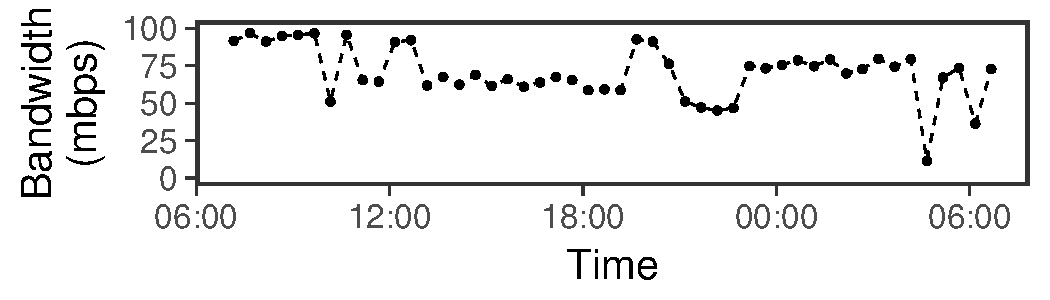
\includegraphics[width=\textwidth]{figures/aws-variation.pdf}
      \caption{Bandwidth variations throughout the day between Amazon EC2
        sites. Similar scarcity and variation for wireless networks, broadband
        access networks and cellular networks
        (\hyperlink{cellular-variation}{backup slides}).}
    \end{figure}
  }

  % \visible<5>{
  %   \begin{figure}
  %     \begin{subfigure}{0.49\textwidth}
  %       \centering
  %       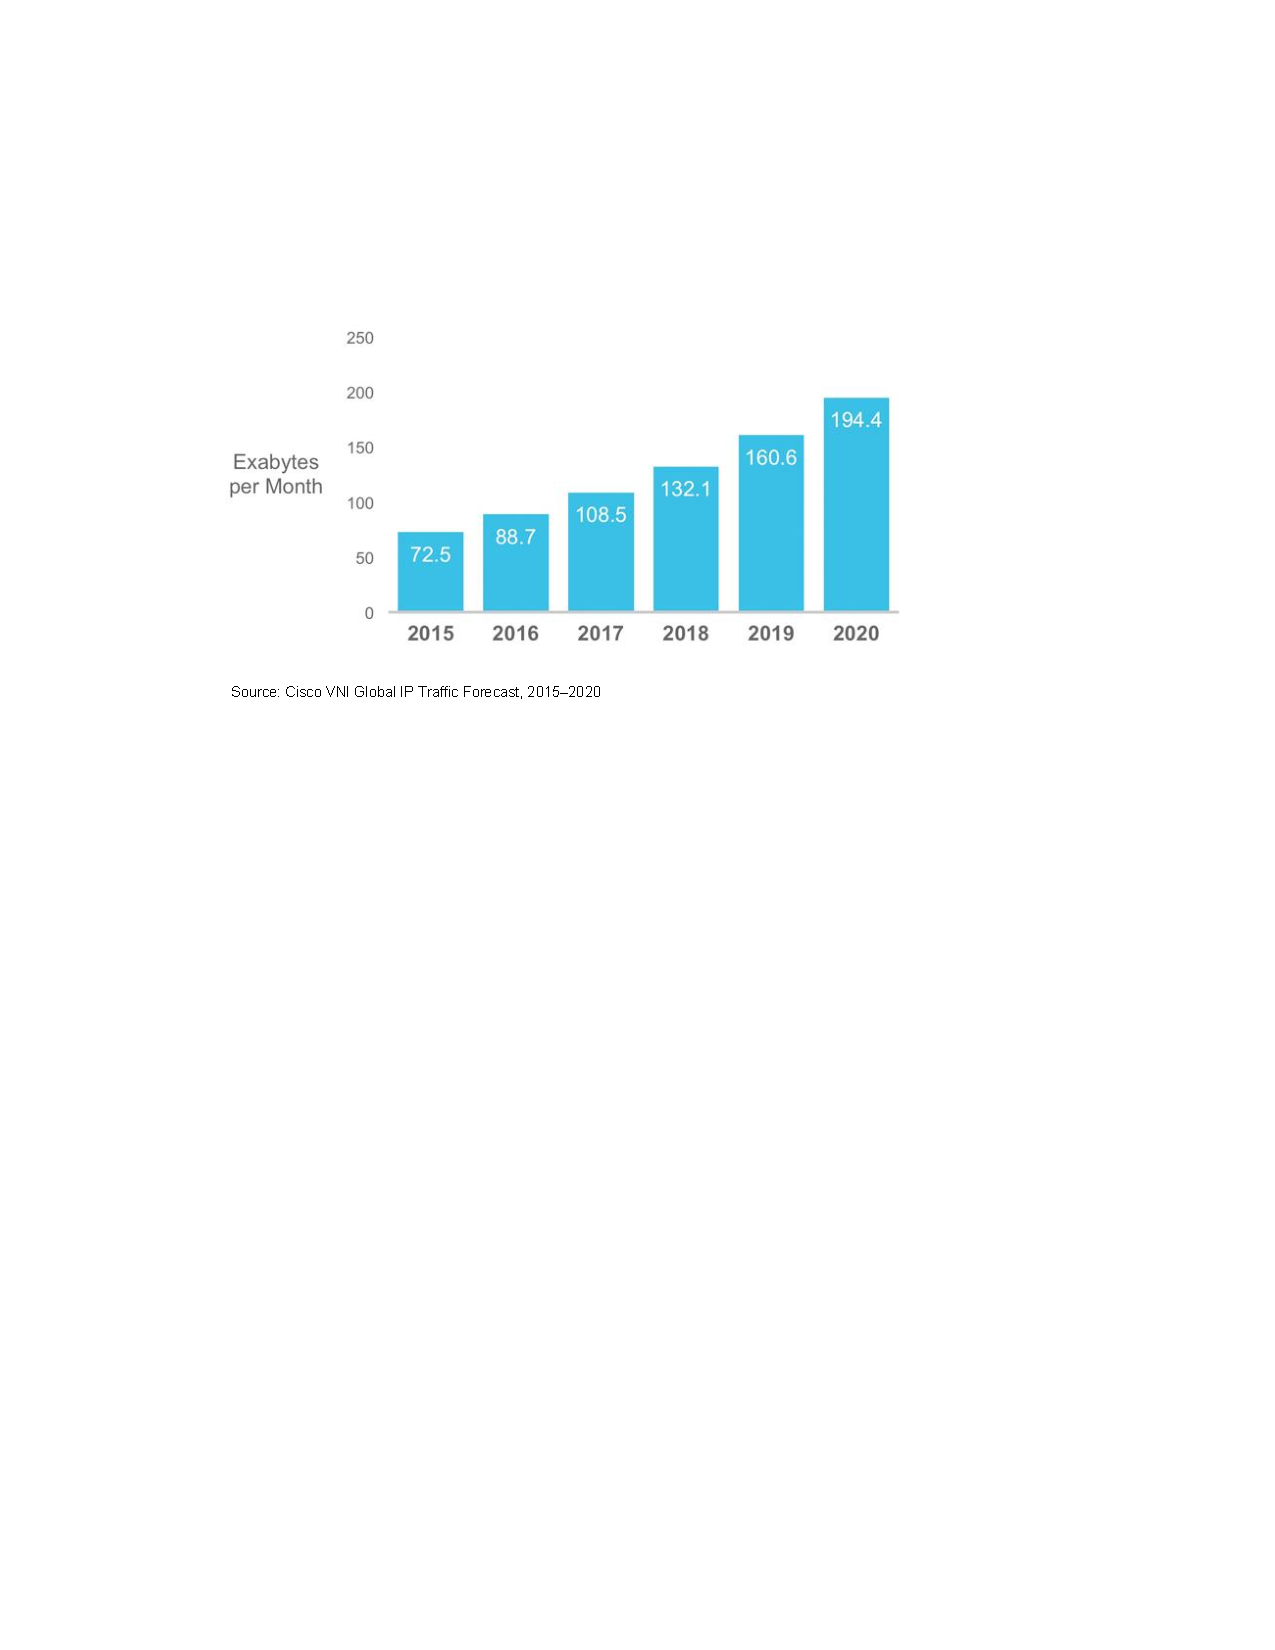
\includegraphics[width=\textwidth]{figures/cisco.pdf}
  %       \caption{Cisco Project Data Growth~\cite{cisco2013zettabyte}}
  %     \end{subfigure}
  %     \hfill
  %     \begin{subfigure}{0.49\textwidth}
  %       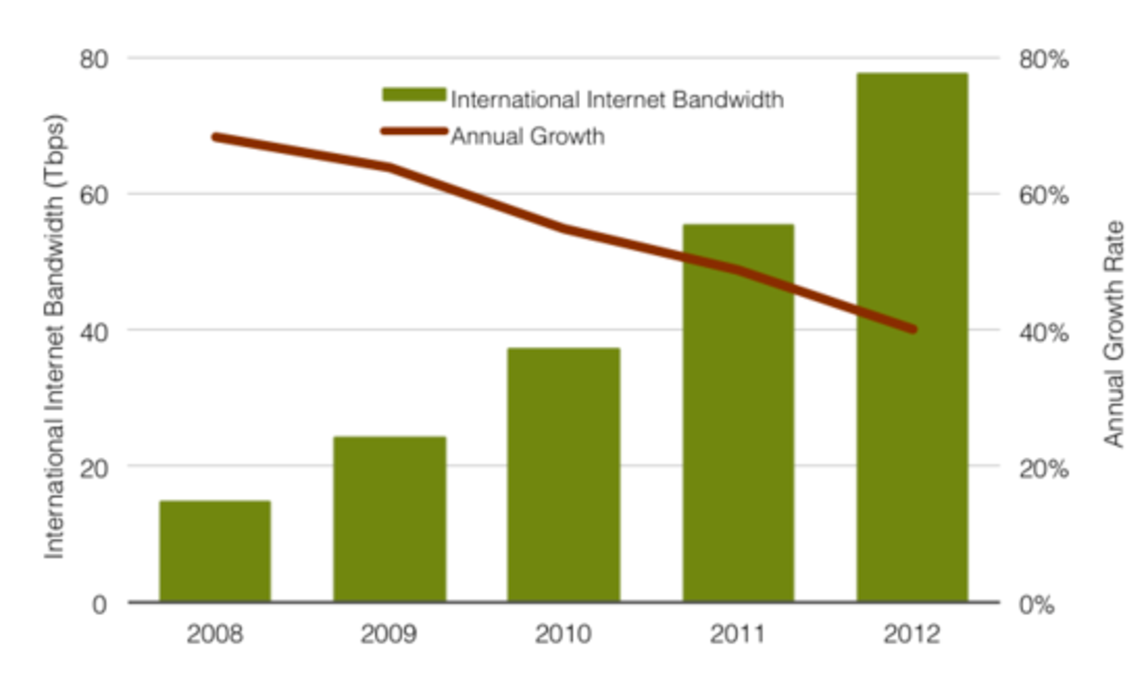
\includegraphics[width=\textwidth]{figures/telegeography.pdf}
  %       \caption{Network backbone capacity growth slows
  %         down~\cite{global2016telegeography}}
  %     \end{subfigure}
  %   \end{figure}
  % }
  \visible<5>{

    What about edge processing? (I will cover in the second half of this talk).

    But communication is not avoidable.

    \begin{itemize}
    \item Large performance gap between the cloud and the edge (GPU/TPU/ASIC).
    \item Aggregation is sometimes necessary in applications.
    \item Last-hop wireless may become the bottleneck.
    \end{itemize}
  }

\end{frame}

\begin{frame}[t]{Fidelity vs.\,Freshness}
  When the network resource is not sufficient:

  \begin{itemize}
  \item TCP ensures data delivery, but hurts latency
  \item UDP sends as fast as possible, uncontrolled packet loss
  \only<2->{
  \item Manual policies (developer heuristics) are sub-optimal
  }
  \only<3>{
      \begin{itemize}
      \item JetStream~\cite{rabkin2014aggregation} uses manual policy
      \item ``if bandwidth is insufficient, switch to sending images at 75\% fidelity,
        then 50\% if still not enough''
      \end{itemize}
    }
  \only<4->{\item Application-specific optimizations don't generalize}
    \only<5>{
      \begin{itemize}
      \item Video streaming often aims at Quality of Experience (limited
        degradation dimension, e.g. maintain 25FPS)
      \item For object detection, resolution matters more than FPS
      \end{itemize}
    }
  \end{itemize}

  \only<7>{
    \begin{figure}
      \centering
      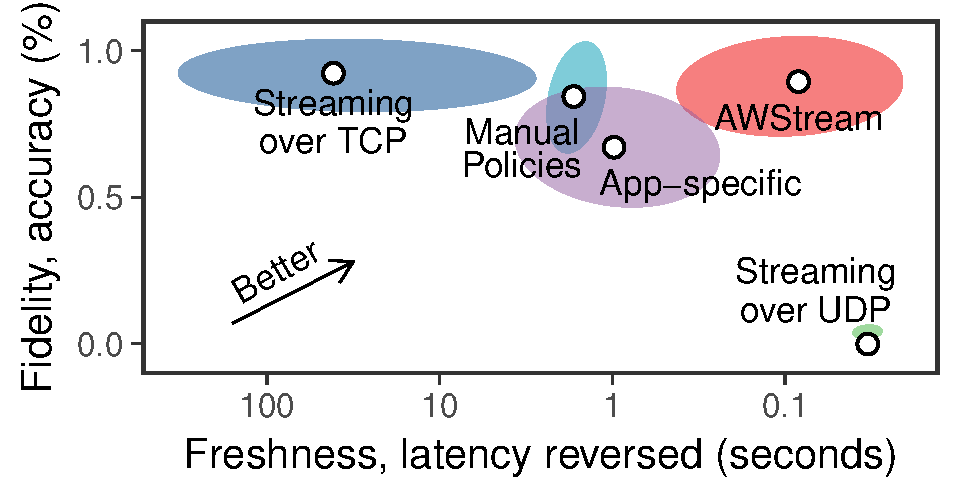
\includegraphics[width=0.8\columnwidth]{figures/fidelity-freshness.pdf}
    \end{figure}
  }
  \only<8>{
    \begin{figure}
      \centering
      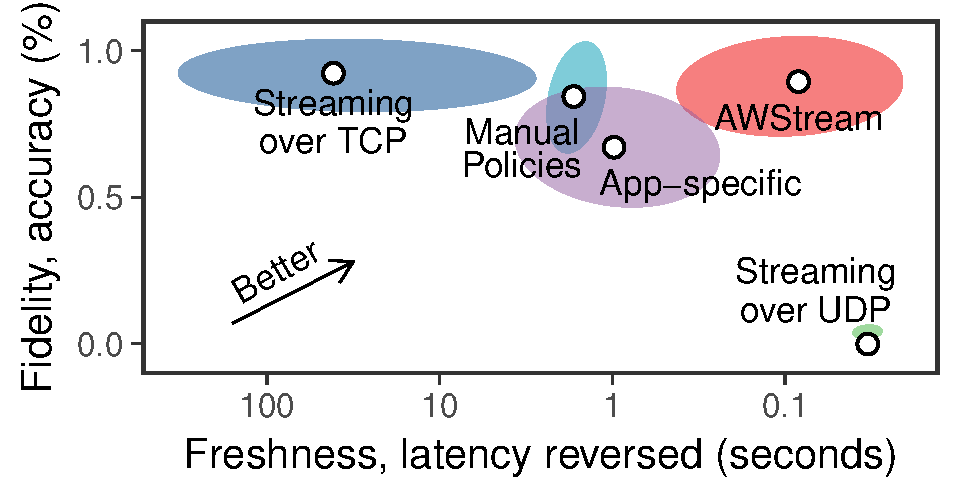
\includegraphics[width=0.8\columnwidth]{figures/fidelity-freshness-full.pdf}
    \end{figure}
  }
\end{frame}

\captionsetup[figure]{labelformat=empty,font=scriptsize,labelfont=scriptsize}
\begin{frame}{Application-specific Optimizations Don't Generalize}
  \pgfplotstableread[row sep=\\,col sep=&]{
    Frame Rate & Bandwidth (normalized) & Accuracy \\
    30 & 100 & 100 \\
    10 & 40 & 92 \\
     5 & 21 & 90 \\
     3 & 13 & 87 \\
     2 & 9 & 84 \\
  }\stationaryframerate
  \pgfplotstableread[row sep=\\,col sep=&]{
    Resolution & Bandwidth (normalized) & Accuracy \\
    1080p & 100 & 100 \\
    900p & 79 & 87 \\
    720p & 54 & 84 \\
    540p & 29 & 71 \\
    360p & 17 & 11 \\
  }\stationaryresolution

  \begin{columns}[t]
    \vspace{1em}
    \column{0.4\textwidth}
    \begin{figure}
      \centering
      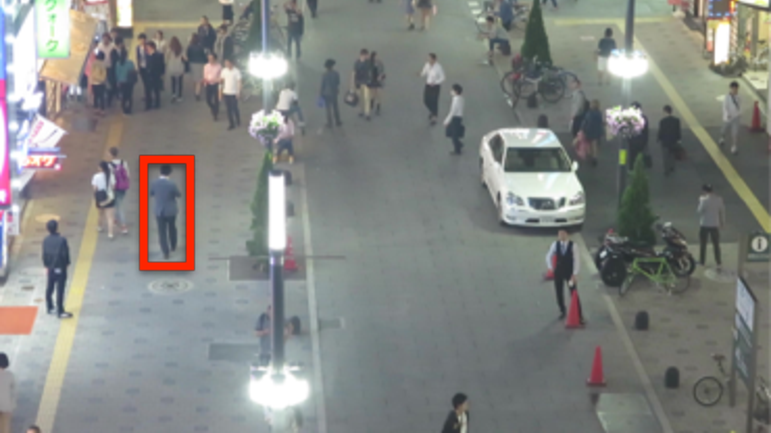
\includegraphics[width=\linewidth]{figures/mot-1.pdf}
      \caption{t=0s, small target in far-field views}
    \end{figure}
    \vspace{-1em}
    \begin{figure}
      \centering
      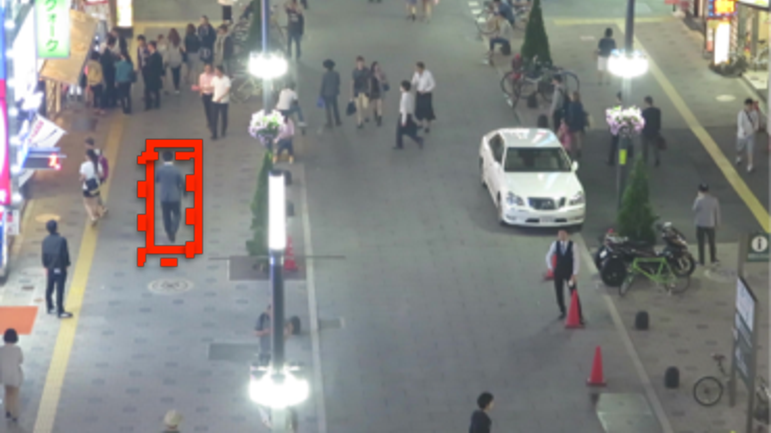
\includegraphics[width=\linewidth]{figures/mot-2.pdf}
      \caption{t=1s, small difference}
    \end{figure}

    \column{0.6\textwidth}

    \only<2>{
      Positive if intersection over union (IOU) larger than 0.5.

      \[
        \text{IOU} = \frac{\text{Area of Intersection}}{\text{Area of Union}}
      \]

      \begin{figure}
        \begin{subfigure}{0.3\textwidth}
          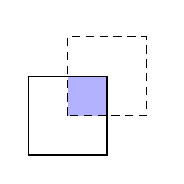
\begin{tikzpicture}
            \fill[color=blue!30] (0.5, 0.5) rectangle (1, 1);
            \node[draw=none] () at (1.5, 1.5) {};
            \draw (0, 0) rectangle (1, 1);
            \draw[densely dashed] (0.5, 0.5) rectangle (1.5, 1.5);
          \end{tikzpicture}
          \caption{IOU=0.14}
        \end{subfigure}
        \begin{subfigure}{0.3\textwidth}
          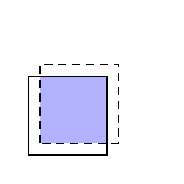
\begin{tikzpicture}
            \fill[color=blue!30] (0.15, 0.15) rectangle (1, 1);
            \node[draw=none] () at (1.5, 1.5) {};
            \draw (0, 0) rectangle (1, 1);
            \draw[densely dashed] (0.15, 0.15) rectangle (1.15, 1.15);
          \end{tikzpicture}
          \caption{IOU=0.57}
        \end{subfigure}
        \begin{subfigure}{0.3\textwidth}
          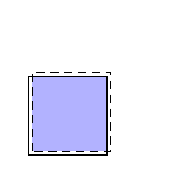
\begin{tikzpicture}
            \fill[color=blue!30] (0.05, 0.05) rectangle (1, 1);
            \node[draw=none] () at (1.5, 1.5) {};
            \draw[densely dashed] (0.05, 0.05) rectangle (1.05, 1.05);
            \draw (0, 0) rectangle (1, 1);
          \end{tikzpicture}
          \caption{IOU=0.82}
        \end{subfigure}
      \end{figure}
    }

    \only<3>{

      F1 score is the harmonic mean of precision and recall, \alert{ranging from
        0 to 1}:

      \begin{table}
        \centering
        \begin{tabular}{| c | c | c |}
          \hline
          & P & N \\
          \hline
          Y & True Positive & False Positive \\
          \hline
          N & False Negative & True Negative \\
          \hline
        \end{tabular}
      \end{table}

      \begin{equation*}
        \begin{split}
          \text{Precision} &= \frac{\text{true positive}}{\text{all positive}} \\
          \text{Recall} &= \frac{\text{true positive}}{\text{all detection}} \\
          \text{F1} &= \frac{2}{\frac{1}{\text{Recall}} + \frac{1}{\text{Precision}}}
        \end{split}
      \end{equation*}

    }
    \only<4->{
      \begin{tikzpicture}
        \tikzstyle{every node}=[font=\footnotesize]
        \begin{axis}[
          ybar,
          bar width               = .4cm,
          width                   = 1.1\textwidth,
          height                  = 0.4\textheight,
          legend style            = {at = {(0.5, 1.4)}, anchor = north,legend columns = -1},
          symbolic x coords       = {30, 10, 5, 3, 2},
          xtick                   = data,
          enlarge x limits        = 0.15,
          ymin                    = 0,
          ymax                    = 130,
          xlabel                  = {Frame Rate},
          nodes near coords,
          nodes near coords align = {vertical},
          ]
          \addplot+[visible on=<6->] table[x=Frame Rate,y=Bandwidth (normalized)]{\stationaryframerate};
          \addplot+[visible on=<5->] table[x=Frame Rate,y=Accuracy]{\stationaryframerate};
          \legend{Bandwidth (normalized), Accuracy}
        \end{axis}
      \end{tikzpicture}

      \vspace{1em}

      \visible<7>{
        \begin{tikzpicture}
          \tikzstyle{every node}=[font=\footnotesize]
          \begin{axis}[
            ybar,
            bar width               = .4cm,
            width                   = 1.1\textwidth,
            height                  = 0.4\textheight,
            symbolic x coords       = {1080p, 900p, 720p, 540p, 360p},
            xtick                   = data,
            enlarge x limits        = 0.15,
            nodes near coords,
            nodes near coords align = {vertical},
            ymin                    = 0,
            ymax                    = 130,
            xlabel                  = {Resolution},
            ]
            \addplot table[x = Resolution, y = Bandwidth (normalized)]{\stationaryresolution};
            \addplot table[x = Resolution, y = Accuracy]{\stationaryresolution};
            \legend{}
          \end{axis}
        \end{tikzpicture}
      }
    }
  \end{columns}
\end{frame}


\begin{frame}{Application-specific Optimizations Don't Generalize}
  \captionsetup[figure]{labelformat=empty,font=scriptsize,labelfont=scriptsize}

  \pgfplotstableread[row sep=\\,col sep=&]{
    Frame Rate & Bandwidth (normalized) & Accuracy \\
    30 & 100 & 100 \\
    10 & 65 & 64 \\
    5 & 46 & 32 \\
    3 & 34 & 18 \\
    2 & 27 & 10 \\
  }\mobileframerate
  \pgfplotstableread[row sep=\\,col sep=&]{
    Resolution & Bandwidth (normalized) & Accuracy \\
    1080p & 100 & 100 \\
    900p & 69 & 99 \\
    720p & 49 & 97 \\
    540p & 33 & 93 \\
    360p & 22 & 87 \\
  }\mobileresolution

  \begin{columns}[t]
    \column{0.4\textwidth}
    \vspace{2em}
    \begin{figure}
      \centering
      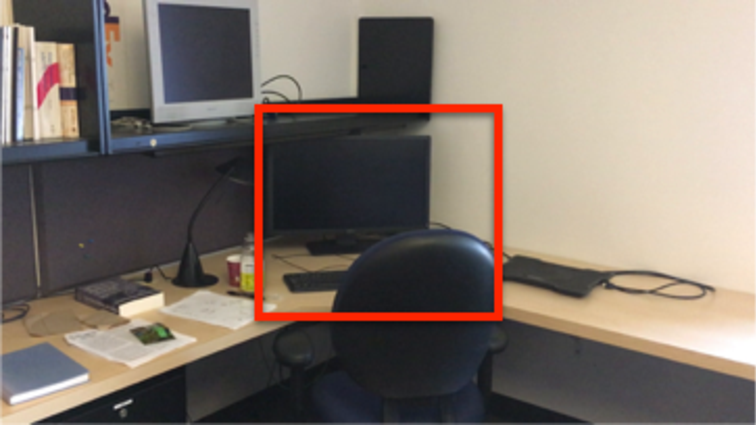
\includegraphics[width=\linewidth]{figures/darknet-1.pdf}
      \caption{t=0s, nearby and large targets}
    \end{figure}
    \vspace{-1em}
    \begin{figure}
      \centering
      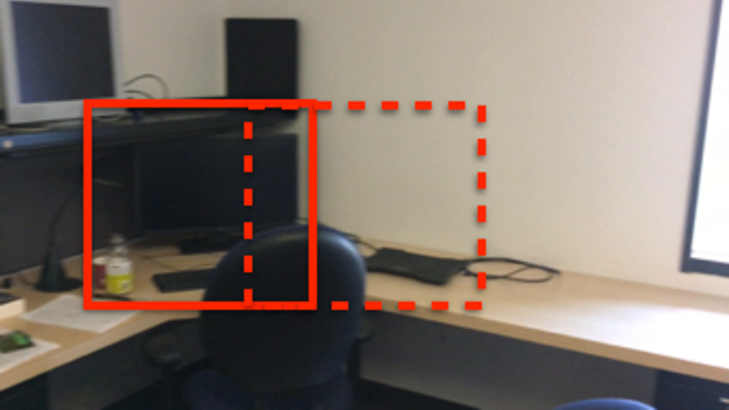
\includegraphics[width=\linewidth]{figures/darknet-2.pdf}
      \caption{t=1s, large difference}
    \end{figure}

    \column{0.6\textwidth}
    \vspace{1.5em}

    \begin{tikzpicture}
      \tikzstyle{every node}=[font=\footnotesize]
      \begin{axis}[
        ybar,
        bar width               = .4cm,
        width                   = 1.1\textwidth,
        height                  = 0.4\textheight,
        legend style            = {at = {(0.5, 1.4)}, anchor = north,legend columns = -1},
        symbolic x coords       = {30, 10, 5, 3, 2},
        xtick                   = data,
        enlarge x limits        = 0.15,
        ymin                    = 0,
        ymax                    = 130,
        xlabel                  = {Frame Rate},
        nodes near coords,
        nodes near coords align = {vertical},
        ]
        \addplot table[x=Frame Rate,y=Bandwidth (normalized)]{\mobileframerate};
        \addplot table[x=Frame Rate,y=Accuracy]{\mobileframerate};
        \legend{Bandwidth (normalized), Accuracy}
      \end{axis}
    \end{tikzpicture}

    \vspace{1em}

    \begin{tikzpicture}
      \tikzstyle{every node}=[font=\footnotesize]
      \begin{axis}[
        ybar,
        bar width               = .4cm,
        width                   = 1.1\textwidth,
        height                  = 0.4\textheight,
        symbolic x coords       = {1080p, 900p, 720p, 540p, 360p},
        xtick                   = data,
        enlarge x limits        = 0.15,
        nodes near coords,
        nodes near coords align = {vertical},
        ymin                    = 0,
        ymax                    = 130,
        xlabel                  = {Resolution},
        ]
        \addplot table[x = Resolution, y = Bandwidth (normalized)]{\mobileresolution};
        \addplot table[x = Resolution, y = Accuracy]{\mobileresolution};
        \legend{}
      \end{axis}
    \end{tikzpicture}
  \end{columns}
\end{frame}

\begin{frame}[t]{Making Adaptation Practical is Challenging}
  \vspace{1em}

  \metroset{block=fill}

  \begin{block}{Goal}
    Minimize bandwidth while maximizing application accuracy
  \end{block}

  \only<2-7>{
    \textbf{Challenges}:

    \begin{enumerate}
      \visible<2->{\item Application-specific optimizations don't generalize.}
      \visible<5->{
        \begin{itemize}
        \item APIs: \texttt{maybe} operators to express adaptation.
        \end{itemize}
      }
      \visible<3->{
      \item It requires expertise and manual work to explore multidimensional adaptation.
      }
      \visible<6->{
        \begin{itemize}
        \item Profiling: automatically learn Pareto-optimal strategy with
          multi-dimensional exploration.
        \end{itemize}
      }
      \visible<4->{
      \item The adaptation happens at the runtime.
      }
      \visible<7->{
        \begin{itemize}
        \item Engineering an adaptation system to balance latency and accuracy.
        \end{itemize}
      }
    \end{enumerate}
  }
  \only<8>{
    \begin{figure}
      \centering
      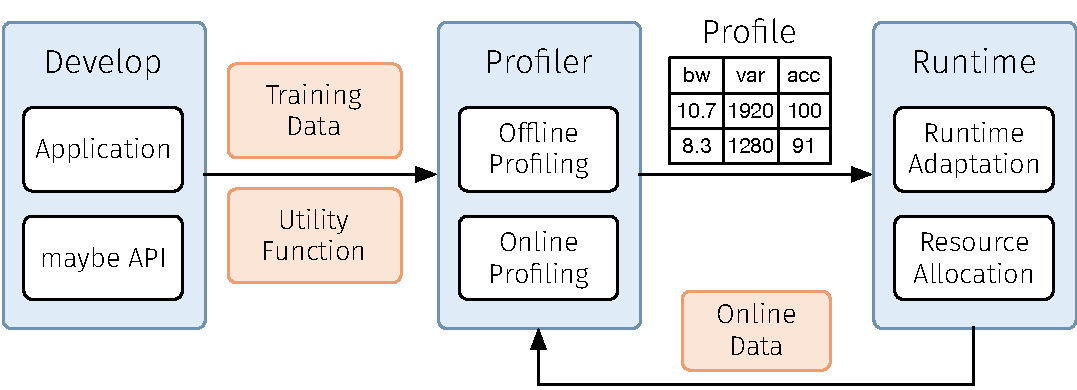
\includegraphics[width=0.8\linewidth]{figures/arch.pdf}
    \end{figure}
  }
\end{frame}

% \begin{frame}{System Architecture Overview}
%   \centering
%   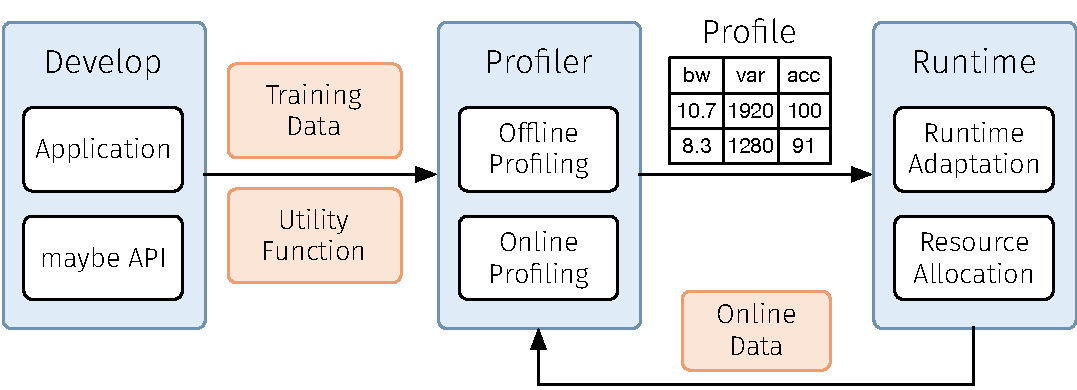
\includegraphics[width=0.8\linewidth]{figures/arch.pdf}\\
%   \begin{tikzpicture}
%     \draw[dashed] (0,0) -- (10,0);
%   \end{tikzpicture}
%   \centering
%   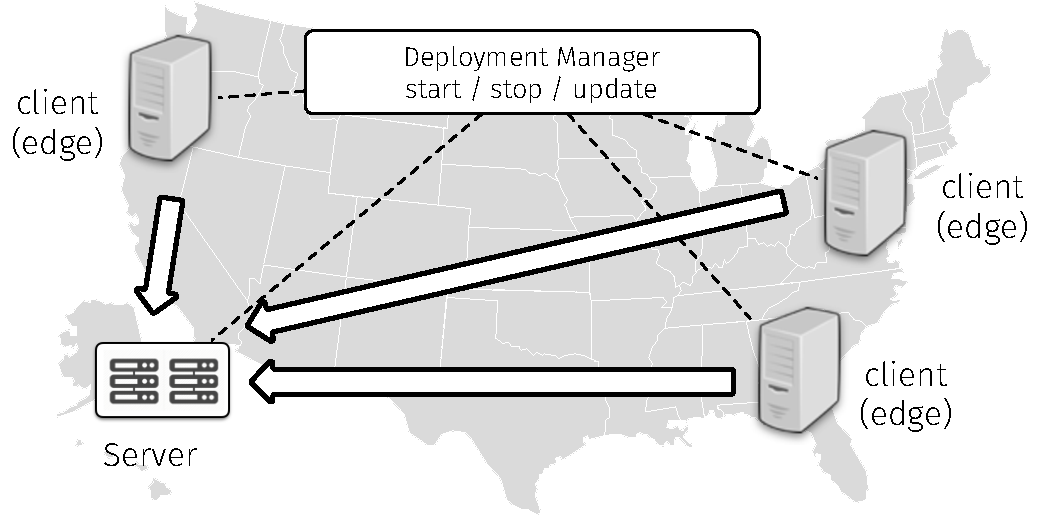
\includegraphics[width=0.7\linewidth]{figures/arch-2.pdf}
% \end{frame}

%%% Local Variables:
%%% mode: latex
%%% TeX-master: "../talk"
%%% TeX-engine: xetex
%%% End:
